\begin{figure}
    \centering
    \begin{minipage}{0.49\linewidth}
        \centering
        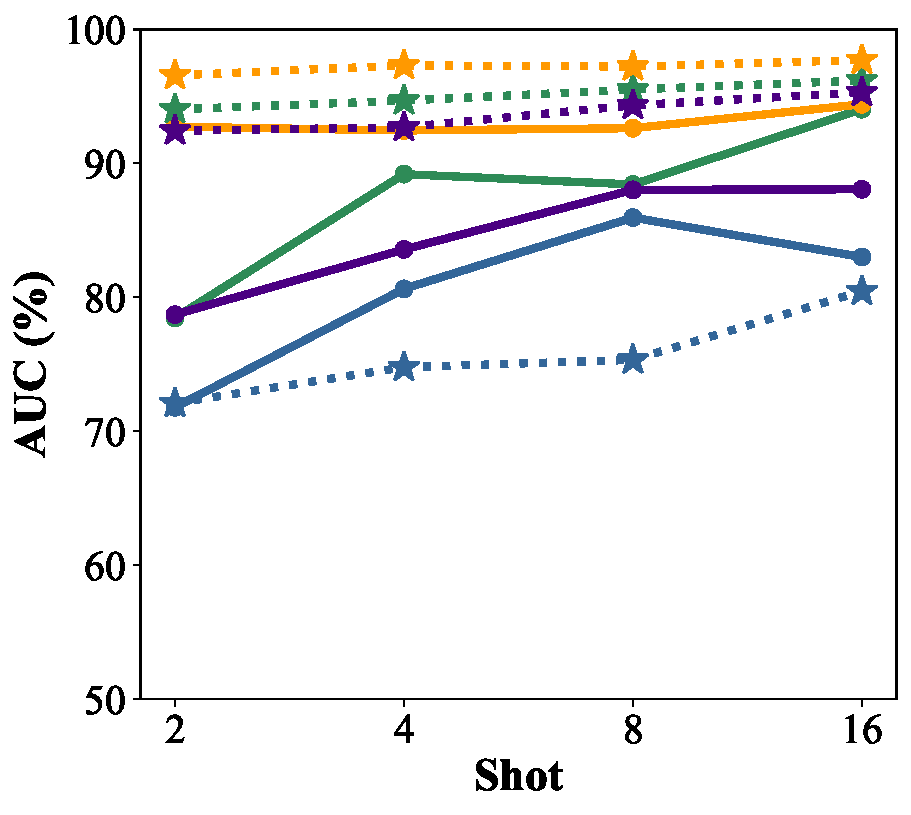
\includegraphics[width=1.0\linewidth]{img/fewshots/Brain.pdf}
        \subcaption*{(a) BrainMRI}
    \end{minipage}
    \begin{minipage}{0.49\linewidth}
        \centering
        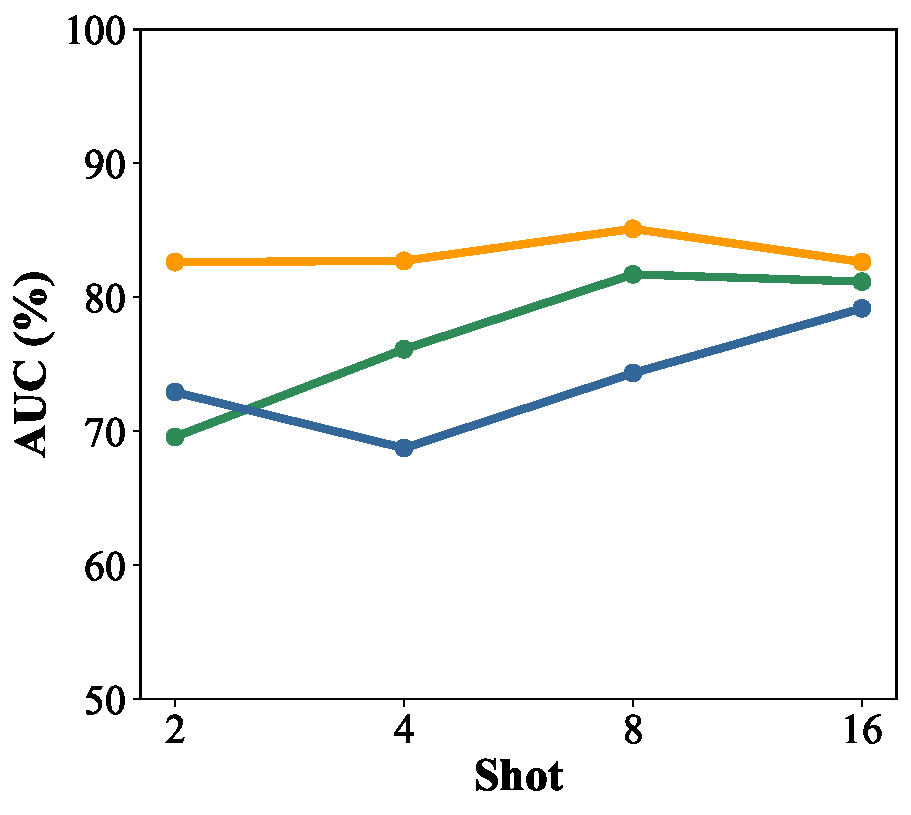
\includegraphics[width=1.0\linewidth]{img/fewshots/Histopathology.pdf}
        \subcaption*{(d) HIS}
    \end{minipage}
    \begin{minipage}{0.49\linewidth}
        \centering
        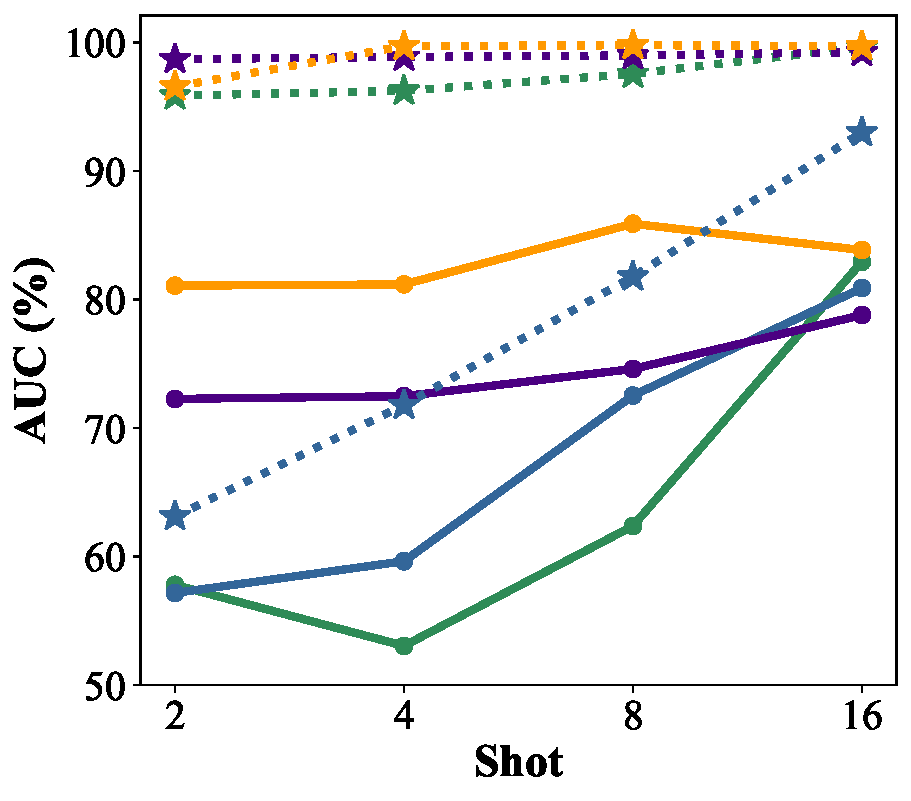
\includegraphics[width=1.0\linewidth]{img/fewshots/Liver.pdf}
        \subcaption*{(b) LiverCT}
    \end{minipage}
    \begin{minipage}{0.49\linewidth}
        \centering
        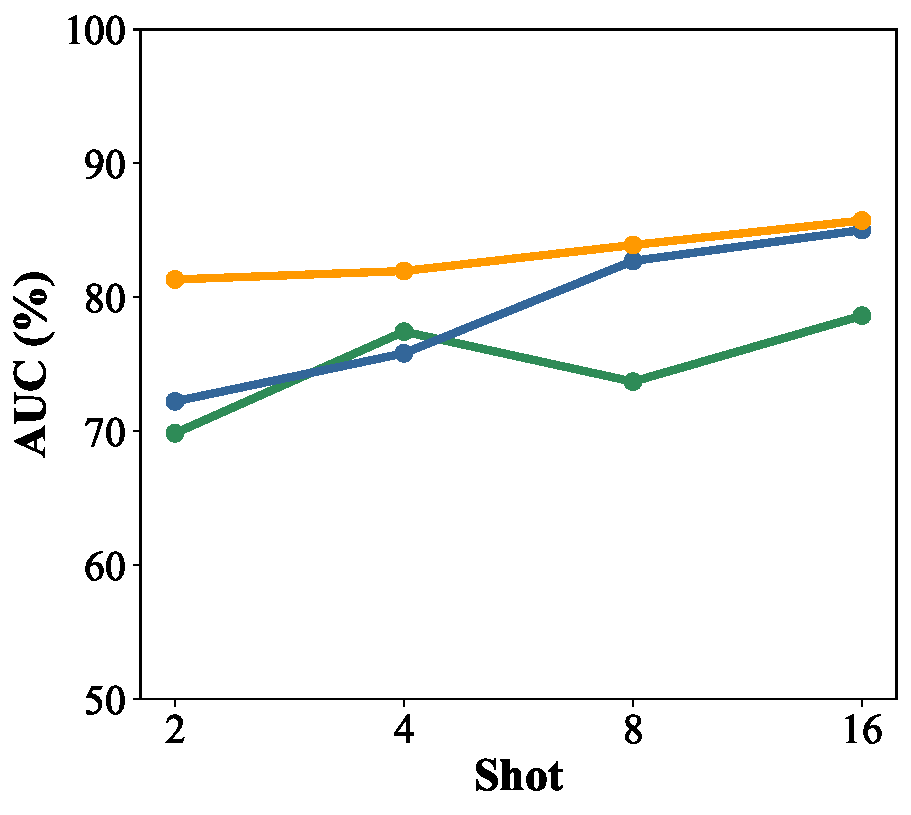
\includegraphics[width=1.0\linewidth]{img/fewshots/Chest.pdf}
        \subcaption*{(e) ChestXray}
    \end{minipage}
    \begin{minipage}{0.49\linewidth}
        \centering
        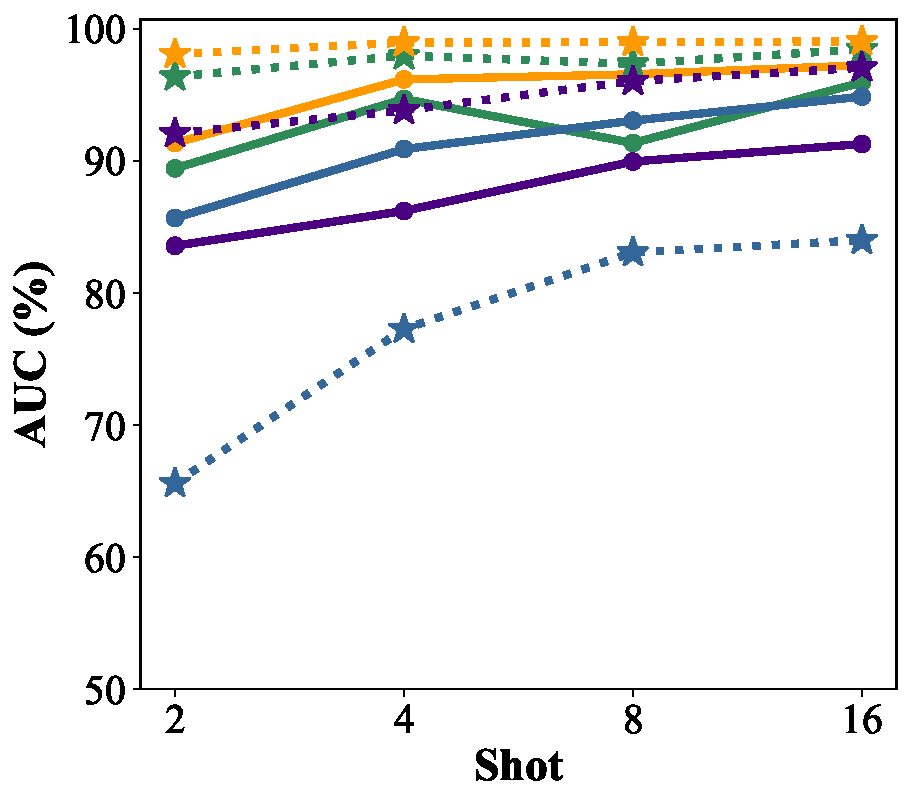
\includegraphics[width=1.0\linewidth]{img/fewshots/Retina_RESC.pdf}
        \subcaption*{(c) RESC}
    \end{minipage}
    \begin{minipage}{0.49\linewidth}
        \centering
        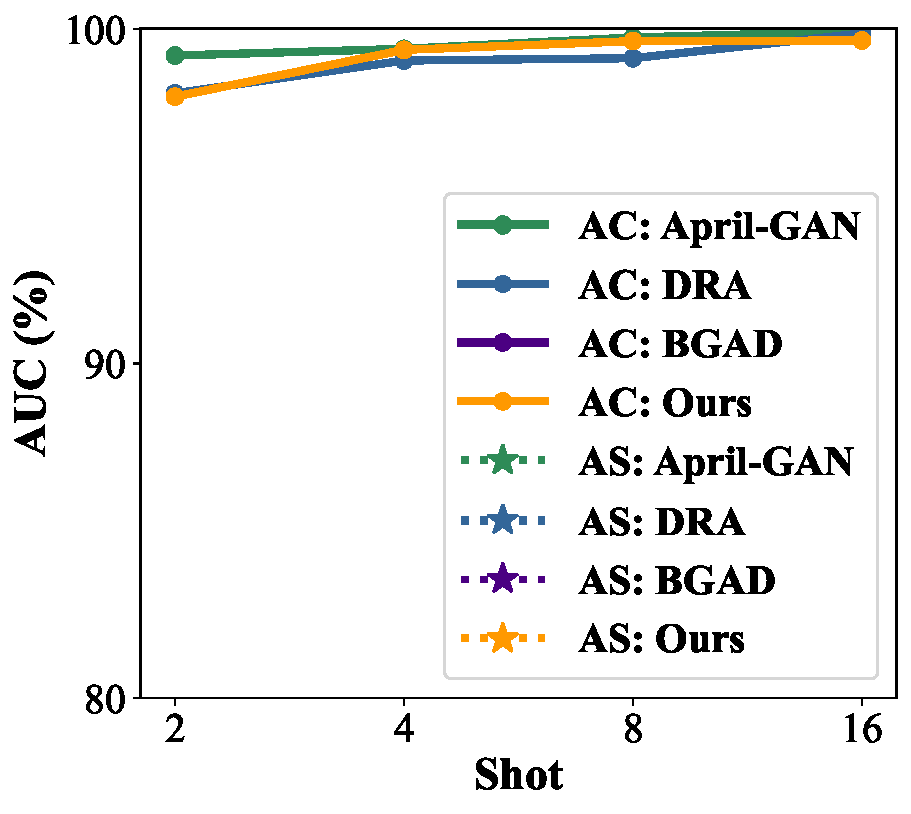
\includegraphics[width=1.0\linewidth]{img/fewshots/Retina_OCT2017.pdf}
        \subcaption*{(f) OCT17}
    \end{minipage}
    \vspace{-3pt}
    \caption{Comparisons with state-of-the-art \textbf{few-shot} anomaly detection methods on datasets of (a) BrainMRI, (b) LiverCT, (c) RESC, (d) HIS, (e) ChestXray, and (f) OCT17, with the shot number $K=\{2,4,8,16\}$. The AUCs (in \%) for anomaly classification (AC) and anomaly segmentation (AS) are reported. More details are included in Appendix~\ref{sec:ap_results}. 
    }
    \vspace{-4em}
    \label{fig:fewshot}
\end{figure}

\section{Experiments}
\label{sec:exp}

\subsection{Experimental Setups}
\noindent\textbf{Datasets.}
We consider a medical anomaly detection (AD) benchmark based on BMAD~\cite{bao2023bmad}, covering five distinct medical domains and resulting in six datasets. These include brain MRI~\cite{baid2021rsna,bakas2017advancing,menze2014multimodal}, liver CT~\cite{landman2015miccai,bilic2023liver}, retinal OCT~\cite{hu2019automated,kermany2018identifying}, chest X-ray~\cite{wang2017chestx}, and digital histopathology~\cite{bejnordi2017diagnostic}. Among these, BrainMRI~\cite{baid2021rsna,bakas2017advancing,menze2014multimodal}, LiverCT~\cite{landman2015miccai,bilic2023liver}, and RESC~\cite{hu2019automated} datasets are used for both anomaly classification (AC) and segmentation (AS), while OCT17~\cite{kermany2018identifying}, ChestXray~\cite{wang2017chestx}, and HIS~\cite{bejnordi2017diagnostic} are solely for AC. Detailed descriptions of these datasets are provided in Appendix~\ref{sec:ap_dataset}.

\noindent\textbf{Competing Methods and Baselines.}
In this study, we consider various state-of-the-art AD methods within distinct training settings as competing methods. These settings encompass (i) vanilla methods that use all normal data  (CFlowAD~\cite{gudovskiy2022cflow}, RD4AD~\cite{deng2022anomaly}, PatchCore~\cite{patchcore}, and MKD~\cite{MKD}), (ii) few-normal-shot methods (CLIP~\cite{openclip}, MedCLIP~\cite{wang2022medclip}, WinCLIP~\cite{winclip}), and (iii) few-shot methods (DRA~\cite{DRA}, BGAD~\cite{BGAD}, and April-GAN~\cite{chen2023zero}). We evaluate these methods for AC and AS, excluding BGAD, which is exclusively applied for segmentation due to its requirement for pixel-level annotations during training. 

\noindent\textbf{Evaluation Protocols.} 
The area under the Receiver Operating Characteristic curve metric (AUC) is used to quantify the performance. This metric is a standard in AD evaluation, with separate considerations for image-level AUC in AC and pixel-level AUC in AS.

\noindent\textbf{Model Configuration and Training Details.}
We utilize the CLIP with ViT-L/14 architecture, with input images at a resolution of 240. The model comprises a total of 24 layers, which are divided into 4 stages, each encompassing 6 layers. We use the Adam optimizer at a constant learning rate of 1e-3 and a batch size of 16, conducting 50 epochs for training on one single NVIDIA GeForce RTX 3090 GPU.

\subsection{Comparison with State-of-the-art Methods}
\noindent\textbf{Few-Shot Setting.} In Table~\ref{tal:few}, we compare the performance of MVFA under the few-shot setting with $K=4$ against other state-of-the-art AD methods. For an in-depth analysis of MVFA's performance across various few-shot scenarios ($K\in\{2,4,8,16\}$), please refer to Figure~\ref{fig:fewshot}. MVFA demonstrates superior performance over competing methods like DRA~\cite{DRA}, BGAD~\cite{BGAD}, and April-GAN~\cite{chen2023zero}. Notably, MVFA surpasses April-GAN, the winner of the VAND workshop at CVPR 2023~\cite{vand}, by an average of 7.33\% in AUC for AC and 2.37\% in AUC for AS across all datasets. Compared to BGAD~\cite{BGAD}, MVFA shows an average improvement of 9.18\% in AUC for AC and 3.53\% in AUC for AS, in datasets with pixel-level annotations.

MVFA outperforms few-normal-shot CLIP-based methods such as CLIP~\cite{openclip} and WinCLIP~\cite{winclip}, which also use visual-language pre-trained backbones and employ feature comparisons for AD. MVFA's advantage lies in its ability to effectively utilize a few abnormal samples, leading to significant gains over these methods. For example, against WinCLIP~\cite{winclip}, MVFA achieves an average improvement of 12.60\% in AUC for AC and 2.81\% in AUC for AS across all datasets. While MedCLIP~\cite{wang2022medclip} shows superior results on ChestXray because it was trained on large-scale overlapping ChestXray data in our medical AD benchmark, it lacks broad generalization capabilities, as evidenced by its performance on other datasets.

Moreover, MVFA exhibits substantial improvements over full-normal-shot vanilla AD methods such as CFlowAD~\cite{gudovskiy2022cflow}, RD4AD~\cite{deng2022anomaly}, PatchCore~\cite{patchcore}, and MKD~\cite{MKD}, which rely on much larger datasets than those employed in this study. This highlights the value of incorporating a few abnormal samples as supervision, especially in medical diagnostics where acquiring a limited number of abnormal data can be more practical.

\begin{table}[t]
\centering
\caption{Comparisons with state-of-the-art \textbf{zero-shot} anomaly detection methods with in-/out-domain evaluation. The AUCs (in \%) for AC and AS are reported.}
\vspace{-5pt}
\label{tal:zero}
\small
\scalebox{0.95}{
\setlength{\tabcolsep}{1.0pt}{
\begin{tabular}{C{1.5cm}|C{2.1cm}C{2.2cm}C{2.1cm}}
\toprule
Datasets & WinCLIP~\cite{winclip} & April-GAN~\cite{chen2023zero} & MVFA (ours)\\
\cmidrule(lr){1-4}
HIS & 69.85~/~- & 72.36~/~- & \textbf{77.90}~/~-\\
ChestXray & 70.86~/~- & 57.49~/~- & \textbf{71.11}~/~-\\
OCT17 & 46.64~/~- & 92.61~/~- & \textbf{95.40}~/~-\\
BrainMRI & 66.49~/~85.99 & 76.43~/~\textbf{91.79} & \textbf{78.63}~/~90.27 \\
LiverCT & 64.20~/~96.20 & 70.57~/~97.05 & \textbf{76.24}~/~\textbf{97.85} \\
RESC & 42.51~/~80.56 & 75.67~/~85.23 & \textbf{83.31}~/~\textbf{92.05} \\
\bottomrule
\end{tabular}}}
\end{table}

\begin{table}[t]
    \centering
    \caption{Comparisons with state-of-the-art \textbf{few-shot} anomaly detection methods with K=4 for in-/out-domain evaluation. The AUCs (in \%) for AC/AS are reported.}
    \vspace{-5pt}
\label{tal:in_exp}
    \small
    \scalebox{0.95}{
    \setlength{\tabcolsep}{1.5pt}{
\begin{tabular}{C{2.8cm}|C{1.8cm}C{1.9cm}C{1.7cm}}
\toprule
    AC/AS (avg AUC\%)    &  WinCLIP~\cite{winclip} & April-GAN~\cite{chen2023zero} & MVFA\\
         \cmidrule(lr){1-4}
         in-domain (MVTec) &  95.16/96.27 & 92.77/95.89 & \textbf{96.19}/\textbf{96.32}\\
       out-domain (medical) &  76.38/95.86 & 81.65/96.30 & \textbf{88.97}/\textbf{98.67}\\
       \bottomrule
    \end{tabular}}}
\end{table}

\begin{table*}[t]
\centering
\caption{Ablation studies compared with feature alignment with multi-level projectors and feature adaptation with multi-level adapters under the zero-shot setting. The AUCs (in \%) for AC and AS are reported.}
\label{tal:abl1}
\small
\setlength{\tabcolsep}{2.2pt}{
\begin{tabular}{C{4.0cm}|C{1.3cm}C{1.3cm}C{1.3cm}|C{1.3cm}C{1.3cm}C{1.3cm}C{1.3cm}C{1.3cm}C{1.3cm}}
\toprule
\multirow{2}{*}{Method} & HIS & ChestXray & OCT17 & \multicolumn{2}{c}{BrainMRI} & \multicolumn{2}{c}{LiverCT} & \multicolumn{2}{c}{RESC}\\
\cmidrule(lr){2-10} 
& AC & AC & AC & AC & AS & AC & AS & AC & AS\\
\cmidrule(lr){1-10}
feature alignment (projectors) & 66.32 & 58.06 & 49.85 & 76.66 & 89.39 & 75.85 & 97.64 & 74.44 & 89.17\\
feature adaptation (adapters) & \textbf{77.90} & \textbf{71.11} & \textbf{95.40} & \textbf{78.63} & \textbf{90.27} & \textbf{76.24} & \textbf{97.85} &  \textbf{83.31} & \textbf{92.05}\\
\bottomrule
\end{tabular}}
\end{table*}

\begin{table}[t]
\centering
\caption{Ablation studies of multi-level feature ensemble under \textit{single-level training/multi-level training} with the same model architecture. The average AUCs (in \%) of all six datasets for AC and AS under the few-shot setting (K=4) are reported. Results for each dataset are included in Appendix~\ref{sec:ap_results}.}
\label{tal:abl3}
\small
\scalebox{0.95}{
\setlength{\tabcolsep}{1.2pt}{
\begin{tabular}{C{0.6cm}|C{1.65cm}C{1.65cm}C{1.65cm}C{1.65cm}|C{1.0cm}}
\toprule
& Layer 1 & Layer 2 & Layer 3 & Layer 4 & All\\
\cmidrule(lr){1-6} 
AC & 80.96/83.39 & 88.83/88.84 & 81.25/84.32 & 83.33/84.62 & \textbf{88.97}\\
AS & 97.70/97.98 & 98.58/98.62 & 96.03/98.54 & 97.19/97.44 & \textbf{98.67}\\
\bottomrule
\end{tabular}}}
\end{table}

\noindent\textbf{Zero-Shot Setting.}
The experiments for zero-shot AD were conducted under the \textit{leave-one-out setting}. In this configuration, a designated target dataset was chosen for testing, while the remaining datasets with different modalities and anatomical regions were employed for training. The aim of this approach was to gauge the performance when confronted with unseen modalities and anatomical regions, thereby assessing the model's capacity for generalization. Table~\ref{tal:zero} provides a comprehensive overview of the results pertaining to zero-shot medical AC and AS, offering a comparative evaluation alongside two state-of-the-art methods that also harness the capabilities of the CLIP backbone. MVFA shows remarkable superiority; for instance, it outperforms WinCLIP~\cite{winclip} with an average AUC improvement of 20.34\% for AC and 5.81\% for AS across all datasets. Similarly, against April-GAN~\cite{chen2023zero}, MVFA achieves an average AUC improvement of 6.24\% for AC and 2.03\% for AS across all datasets, underscoring its effectiveness in the challenging zero-shot medical AD setting.

\noindent\textbf{In-Domain Evaluation.} The MVTec AD benchmark~\cite{bergmann2019mvtec}, consisting of 15 industrial defect detection sub-datasets, is considered as in-domain evaluation. As shown in Table~\ref{tal:in_exp}, although our main focus is not in-domain scenarios, MVFA shows comparable performance to state-of-the-art methods in a few-shot setting (K=4). Detailed results for each sub-dataset are included in Appendix~\ref{sec:ap_results}. In our main focus of out-domain evaluations on the medical AD benchmark, MVFA significantly outperforms competing methods, highlighting its superior generalization capabilities.

\subsection{Ablation Studies}\label{sec:abl}

\textbf{Feature Adaptation vs. Feature Alignment.}
We conduct ablation studies in the zero-shot setting for AC and AS to assess the effectiveness of multi-level feature adapters in enhancing cross-modal generalization. For this purpose, we substitute the multi-level feature adapters with distinct multi-level feature projectors, while keeping the parameters and feature alignment loss functions the same. The primary distinction is that each projector is optimized independently, in contrast to the collective optimization approach used for adapters. This ensures that the only variable under consideration is the architecture, while all other factors, including model parameters and training loss functions, remain constant for a valid comparison.

The results, as shown in Table~\ref{tal:abl1}, reveal significant improvements with feature adapters. They lead to substantial improvements in AC, with image-level AUC increasing by 11.58\%, 13.05\%, 45.55\%, 1.97\%, 0.39\%, and 8.87\% for HIS, ChestXay, OCT17, BrainMRI, LiverCT, and RESC, respectively, with an average improvement of 13.57\%. For AS, improvements were observed, with pixel-level AUC increasing by 0.88\%, 0.21\%, and 2.88\% for BrainMRI, LiverCT, and RESC, respectively. These findings highlight the critical role of multi-level feature adapters in boosting the model's generalization capabilities.

\begin{figure}[t]
    \centering    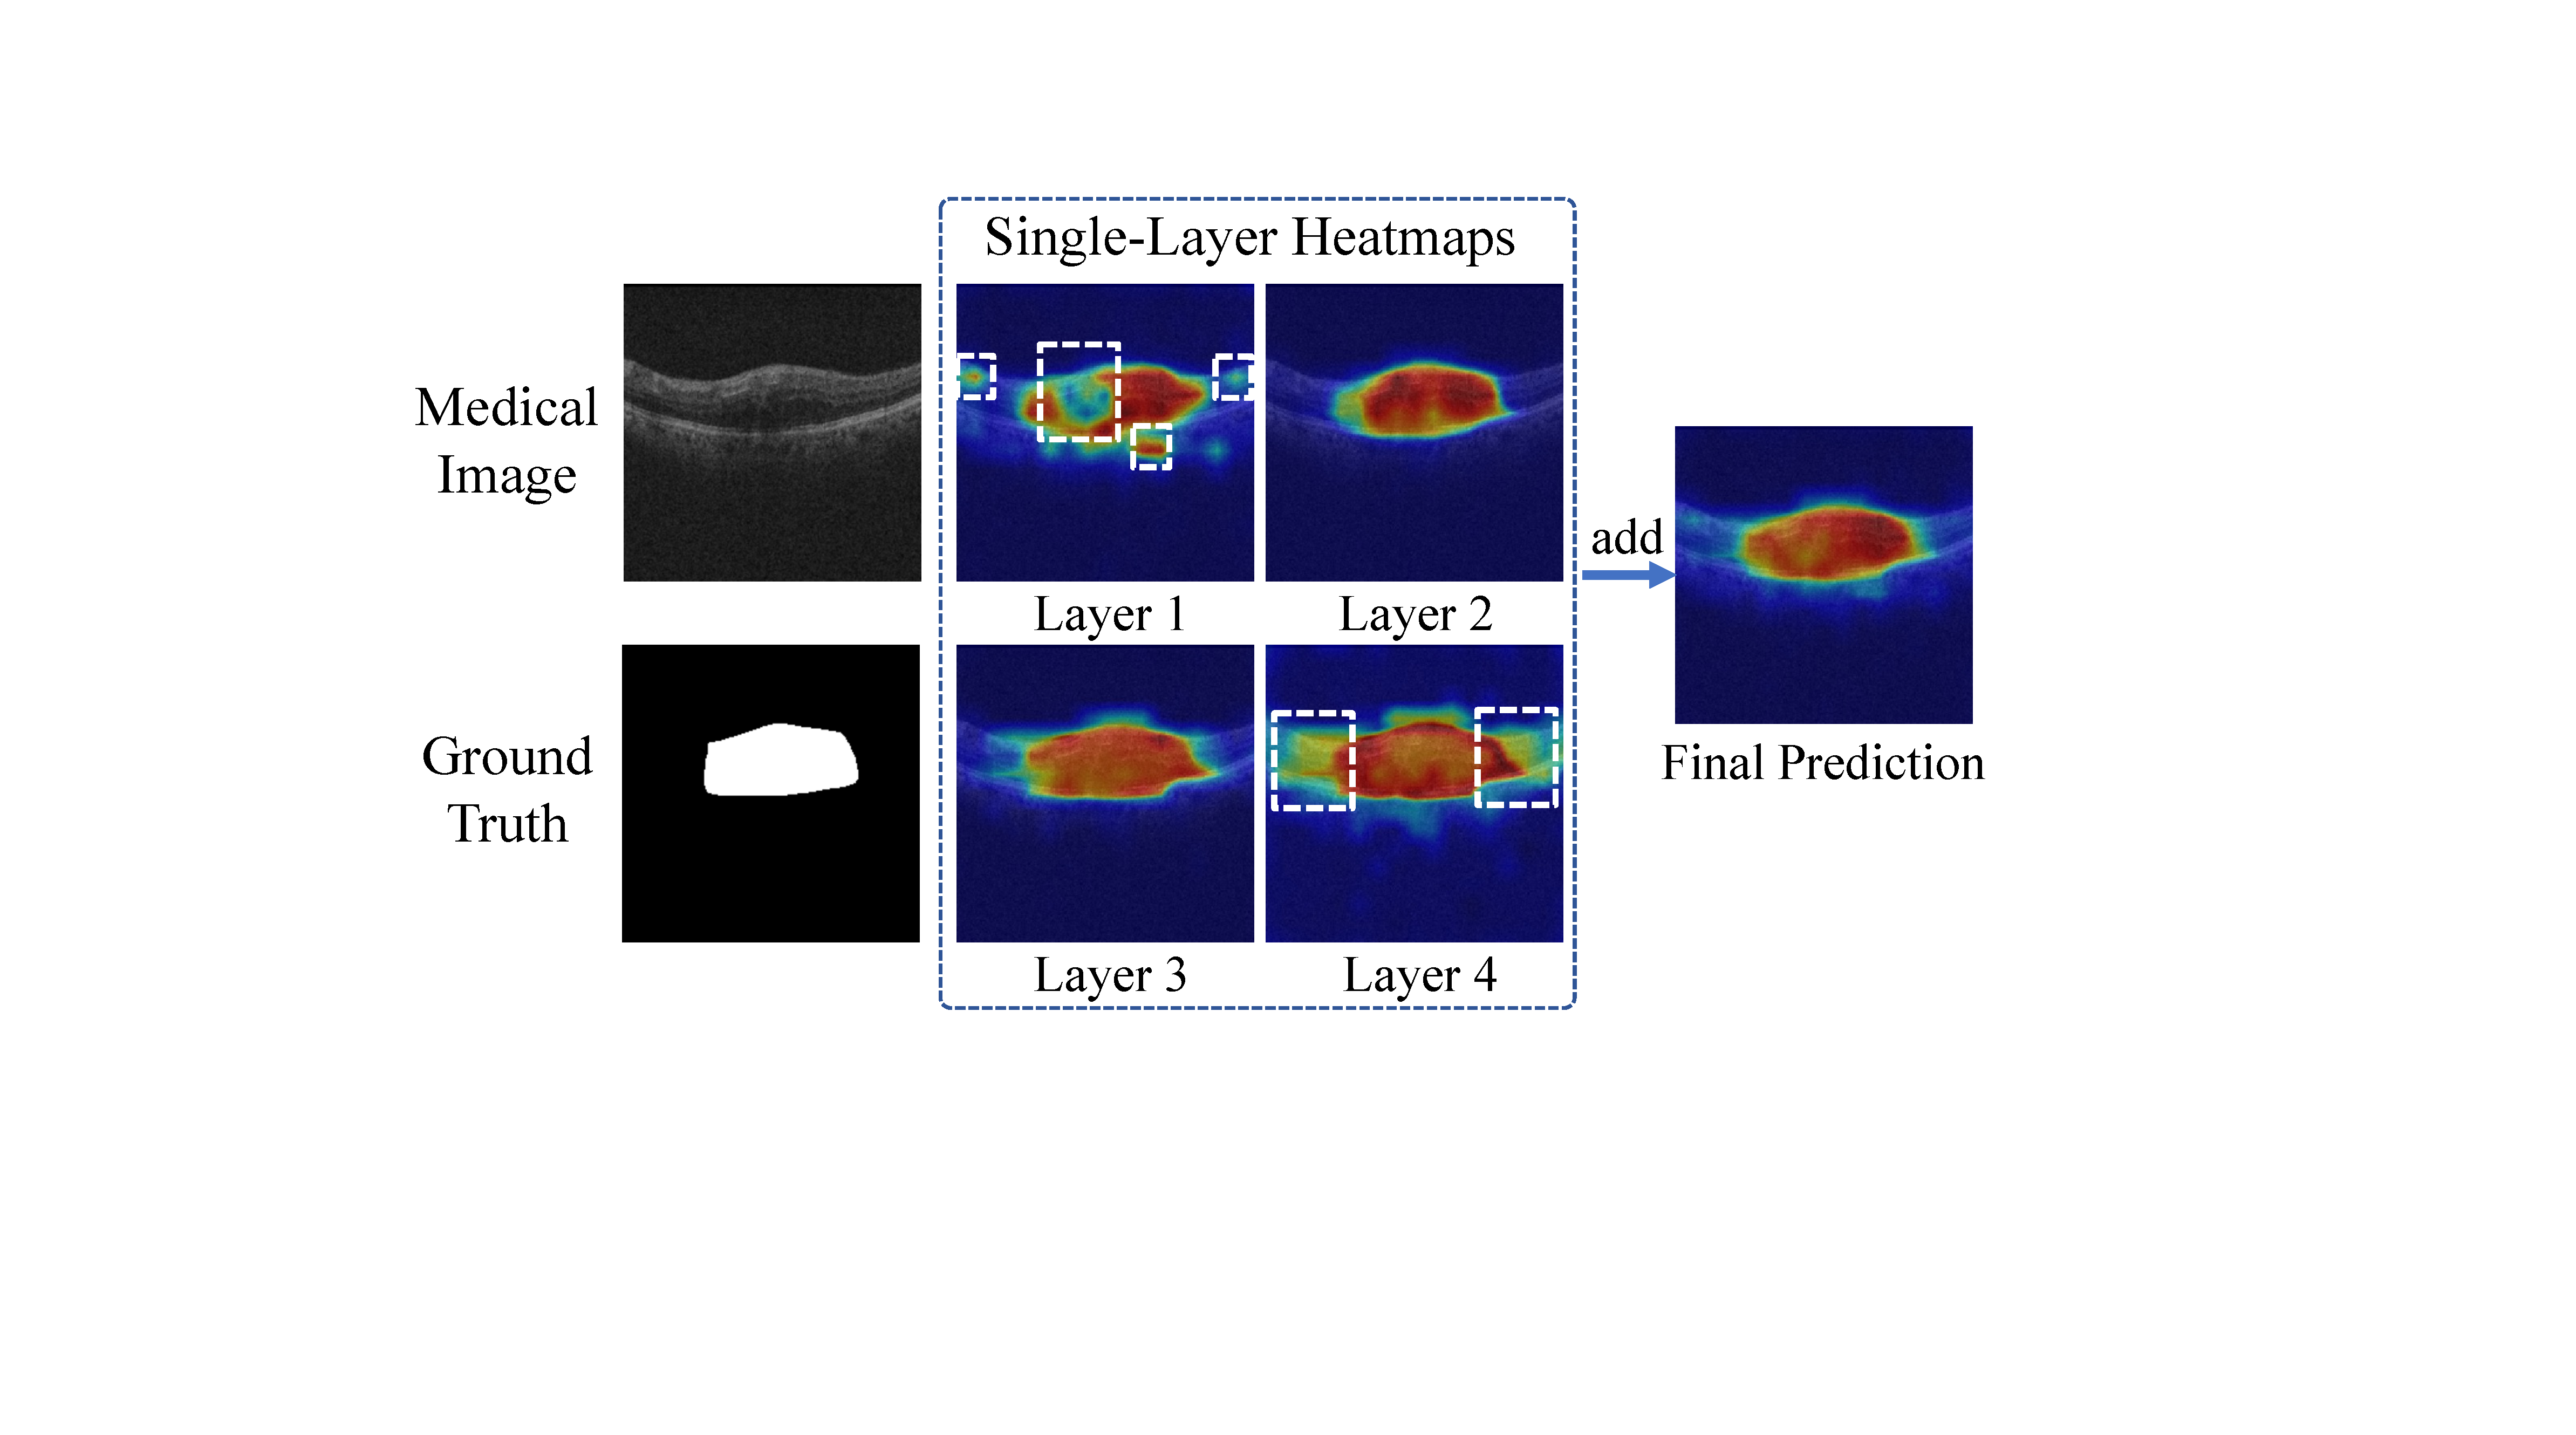
\includegraphics[width=0.48\textwidth]{img/vis_multilayer.pdf}
    \caption{Considering features across multiple levels significantly enhances segmentation performance. The white dashed boxes demarcate regions that have been missed or erroneously segmented. More cases are included in Appendix~\ref{sec:ap_vis}.}
    \label{fig:intro_multilayer}
    \vspace{-5pt}
\end{figure}

\begin{figure*}[t]
    \centering
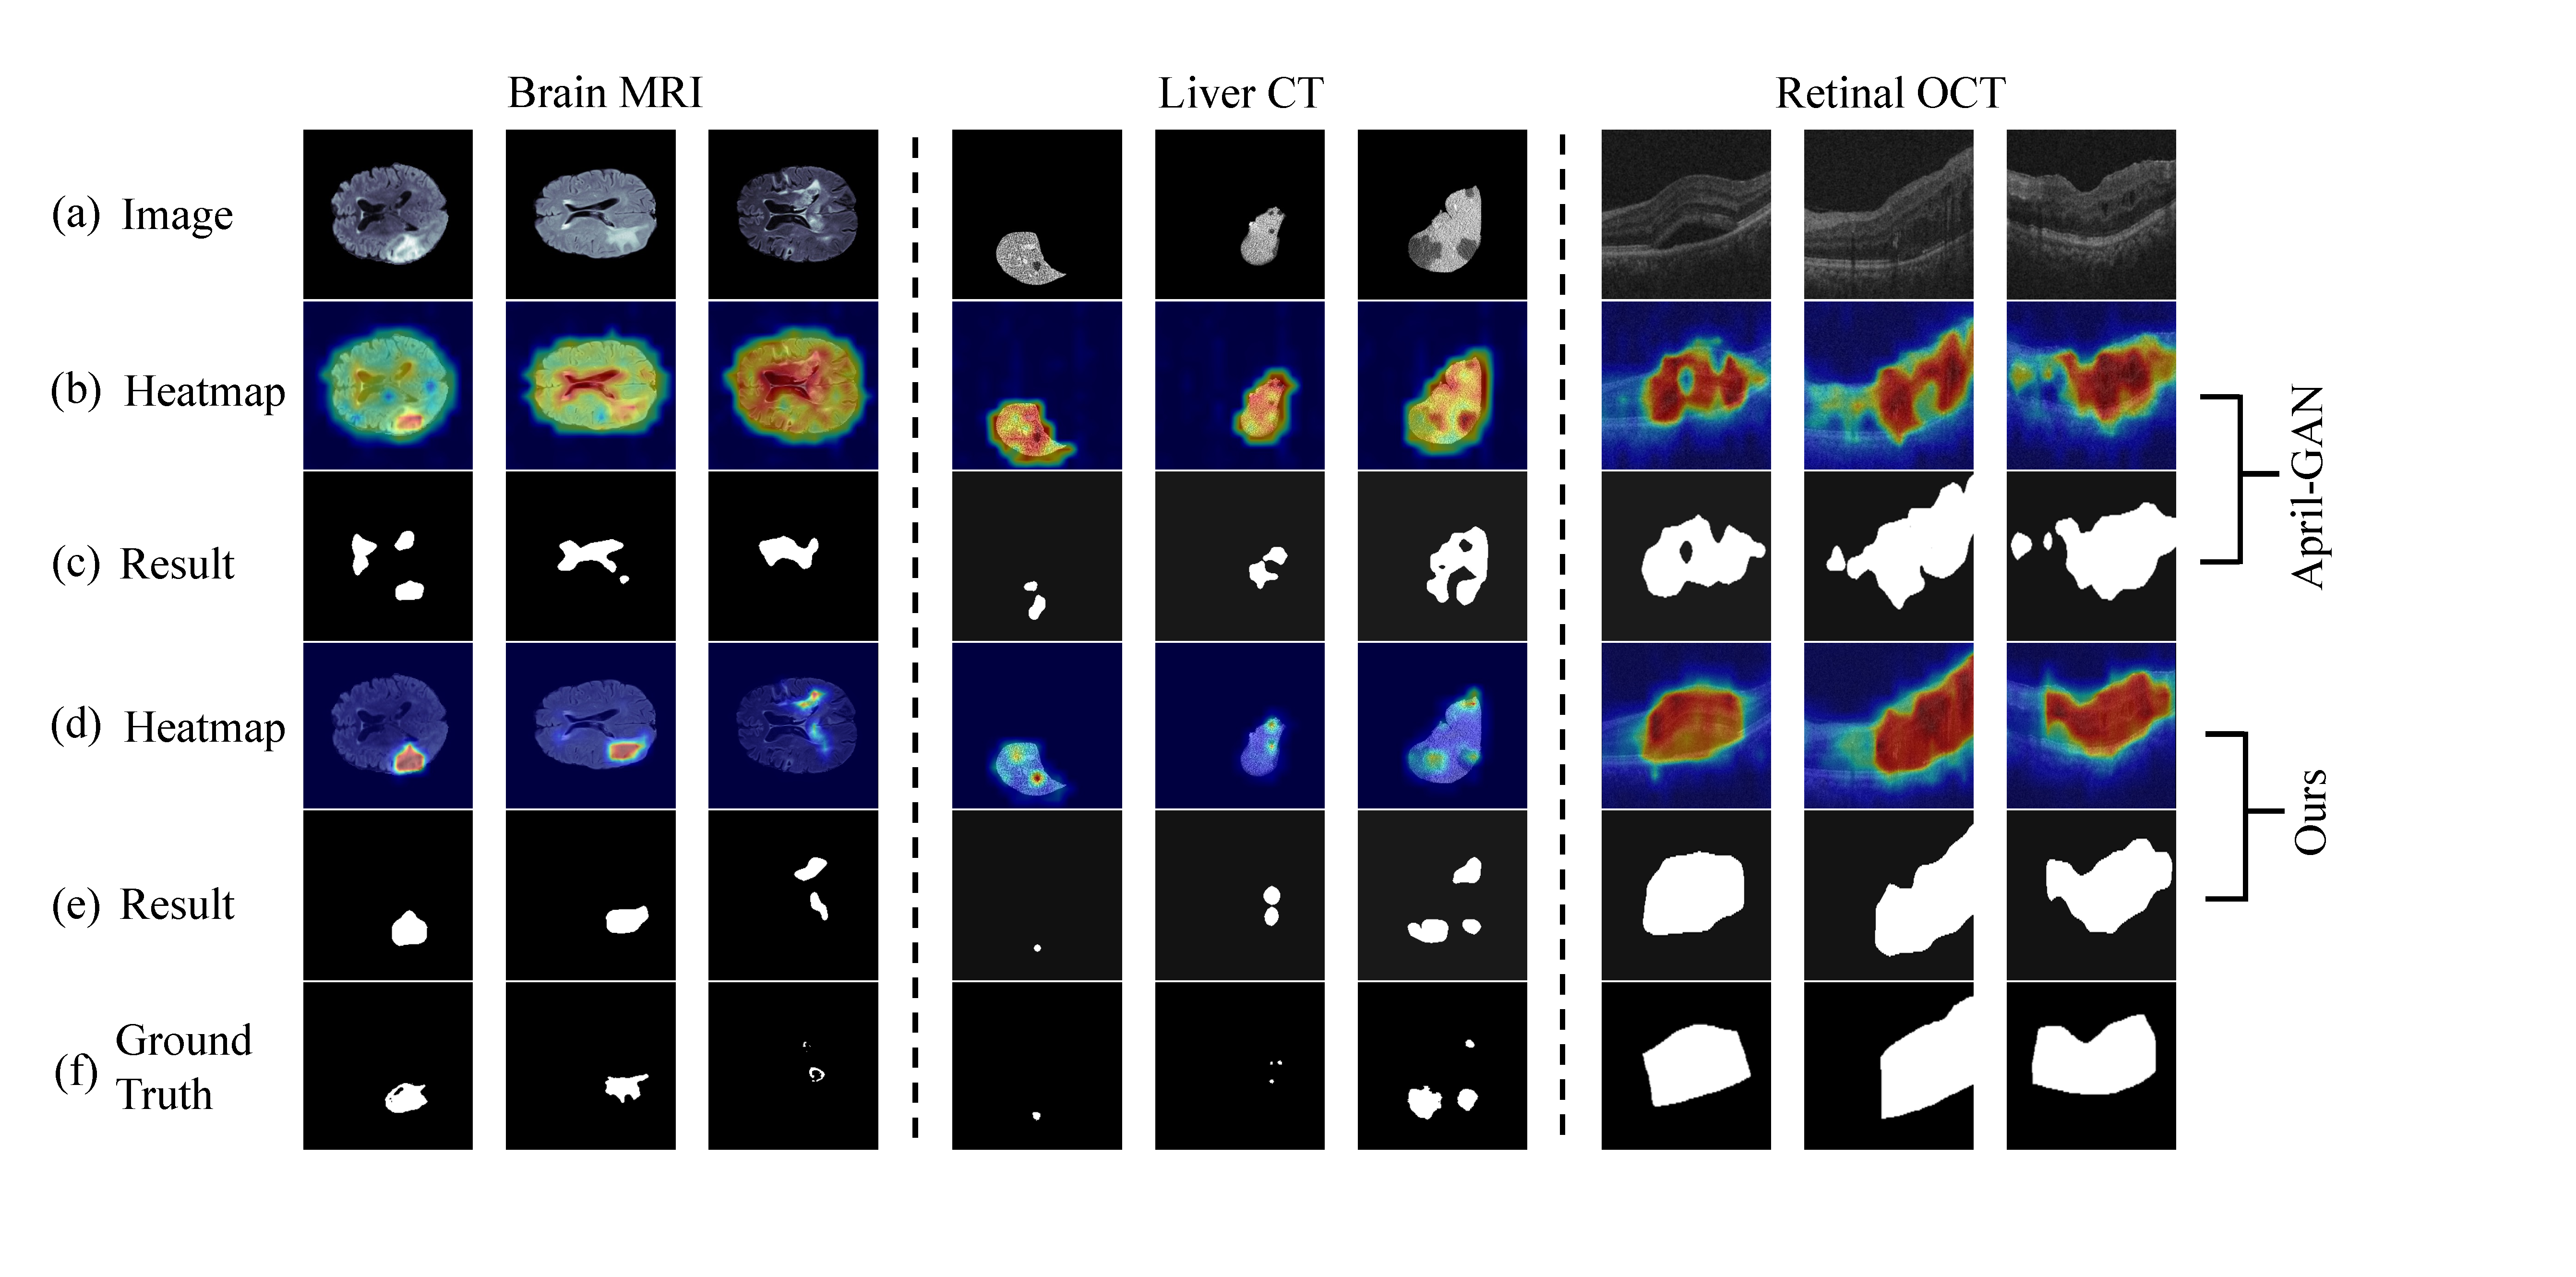
\includegraphics[width=0.9\textwidth]{img/visualize2.pdf}
\vspace{-4pt}
    \caption{Visualization of AS for MVFA on brain MRI, liver CT, and retinal OCT, compared with state-of-the-art method April-GAN. Results from (e) show better performance than results from (c), showing the effectiveness of the proposed multi-level feature adaptation.}
    \label{fig:vis}
    \vspace{-8pt}
\end{figure*}

\begin{figure}[t]
    \centering
    \begin{minipage}{0.49\linewidth}
        \centering
        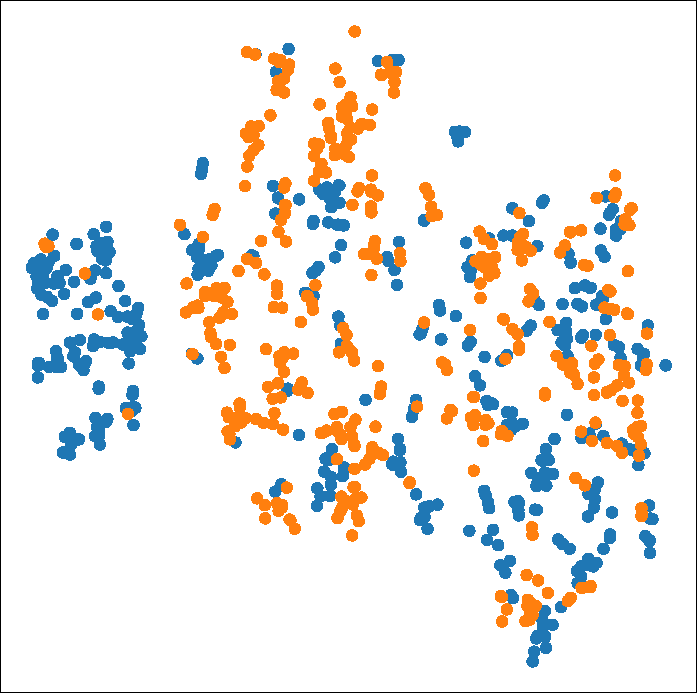
\includegraphics[width=1.0\linewidth]{img/tsne_before.pdf}
        \subcaption*{(a) Without Adapter}
    \end{minipage}
    \begin{minipage}{0.49\linewidth}
        \centering
        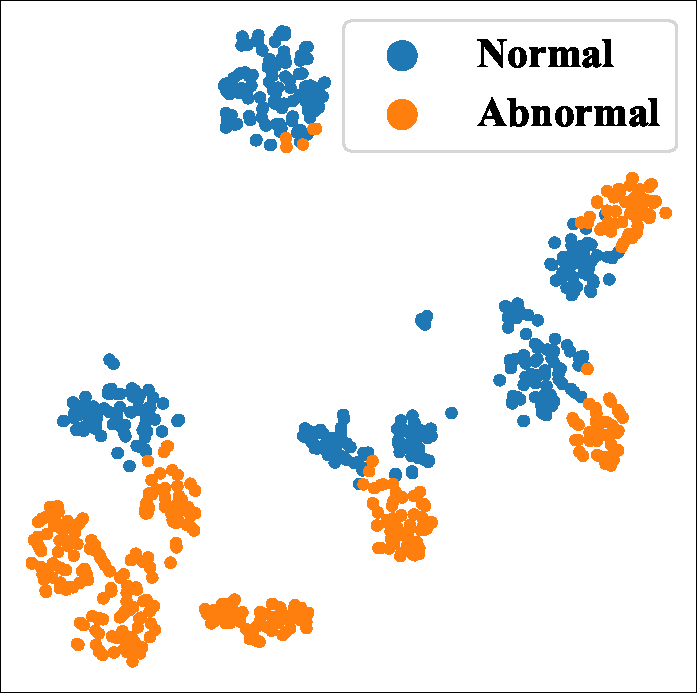
\includegraphics[width=1.0\linewidth]{img/tsne_after.pdf}
        \subcaption*{(b) With Adapter}
    \end{minipage}
    \caption{Visualization, using t-SNE, of the features learned from the RESC test set, using (a) pretrained visual encoder, and (b) multi-level feature adapters. The same t-SNE optimization iterations are used in each case. Results show that features extracted by adapters are separated between normal and abnormal samples.}
    \vspace{-3pt}
    \label{fig:tsne}
\end{figure}

\noindent\textbf{Feature Ensemble in Multi-Level.} 
In this study, as shown in Table~\ref{tal:abl3}, we evaluate the effectiveness of an ensemble approach that integrates features from different layers. The approaches are compared against our comprehensive model, both using the multi-level adapter architecture. Our evaluation specifically focused on features from four distinct layers under two training scenarios: (i) single-layer training, where only one layer's adapter is optimized in each experiment, and (ii) multi-level training, aligning with the methodology of our comprehensive model. The objective of this comparison was to determine the benefits of combining features from multiple layers compared to optimizing each layer's features separately.

The results presented in Table~\ref{tal:abl3} demonstrate that among individual layers, Layer 2 yielded the highest performance, achieving 88.84\% in AC and 98.62\% in AS. However, the ensemble method, which integrates features from all layers, outperformed single-layer approaches, recording AUCs of 88.97\% in AC and 98.67\% in AS. This underscores the effectiveness of combining features from multiple levels. Moreover, multi-level training consistently exceeds the performance of single-layer training, reinforcing the benefits of our multi-level adaptation approach across all layers.

The visualizations of retina anomaly segmentation from various layers, as depicted in Figure~\ref{fig:intro_multilayer}, further reinforce our findings. These visualizations distinctly show that single-layer methods are less effective compared to the ensemble approaches. By synergistically integrating features from different layers, we achieve a marked improvement in AD, which aligns with and supports our quantitative results. 

\subsection{Visualization Analysis}

To qualitatively analyze how the proposed multi-level feature adaptation approach improves anomaly segmentation performance, we visualize the results of several cases from the BrainMRI, LiverCT, and RESC datasets. It can be seen from the results in Figure~\ref{fig:vis} that the segmentation produced by our MVFA (column e) is closer to the ground truth (column f) than that produced by the state-of-the-art method April-GAN (column c). This illustrates the effectiveness of the proposed multi-level visual feature adaptation.

We employ t-SNE~\cite{van2008visualizing} to visualize the learned features from RESC, as depicted in Figure~\ref{fig:tsne}. Each dot corresponds to features of a normal or abnormal sample from the test set. It can be seen that adapter enhances the separation between samples belonging to distinct states, which is beneficial for the identification of AD decision boundaries.